% NOTE:
% latexmk -shell-escape -pvc slides.tex # Watches and compiles on each change.
% latexmk -c slides.tex   # Clean the temporal files.

% NOTE: 
% the minted package doesn't play well with the bibliography!


\documentclass[aspectratio=169]{beamer}

\setbeamertemplate{footline}[frame number]
\beamertemplatenavigationsymbolsempty

% NOTE: Only use numeric for references' style!
\usepackage[backend=biber,style=numeric]{biblatex}
\usepackage{booktabs}
\usepackage{caption}
\usepackage{graphicx}
\usepackage{hyperref}
\usepackage{siunitx}
\usepackage{subcaption}

\addbibresource{slides.bib}  

\captionsetup[figure]{labelformat=empty}

\hypersetup{
    colorlinks,
    allcolors=.,
    urlcolor=blue,
}


\title{Notes on processing large amounts of Earth Observation data}

\author{Alber S\'{a}nchez \href{mailto:alber.ipia@inpe.br}
{alber.ipia@inpe.br}\newline
Guilherme Mataveli}
\institute{
  
\includegraphics[width=4cm,keepaspectratio]{logos/trees-color-h_2.png}
  
\includegraphics[width=1.8cm,keepaspectratio]
  {logos/logoinpe-azul-menor.png} \\
  Research assistant - TreesLab\\National Institute for Space Research - INPE\\
  Brazil
}
\date{\today}



\begin{document}



\frame{\titlepage}

\begin{frame}[allowframebreaks]
    \frametitle{Overview}
    \tableofcontents
\end{frame}



\section{Introduction}



\begin{frame}
    Introduction.
\end{frame}

% \begin{frame}
%     \frametitle{Two stages: developing and processing}
% \end{frame}



\section{Computing concepts}



\begin{frame}
    Computing concepts.
\end{frame}

\begin{frame}
    \frametitle{Hardware}
    \begin{itemize}
        \item Processor.
        \item Memory.
        \item Disc.
    \end{itemize}
\end{frame}

\begin{frame}
    \frametitle{Software}
\end{frame}

\begin{frame}
    \frametitle{Resources}
    \begin{columns}
        \begin{column}{0.5\textwidth}
            \begin{itemize}
                \item \href{https://thecrashcourse.com/topic/computerscience/}
                    {Computer Science} by Crash Course.
            \end{itemize}
        \end{column}
        \begin{column}{0.5\textwidth}
            \begin{figure}
                \centering
                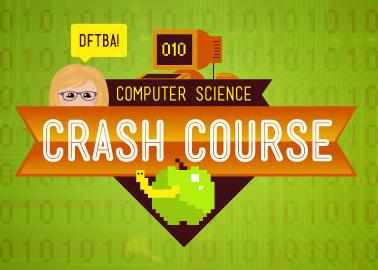
\includegraphics[scale=0.4]
                {img/crash_course_computer_science.jpg}
            \end{figure}
        \end{column}
    \end{columns}
\end{frame}



\section{Linux}



\begin{frame}
    Linux.
\end{frame}

\begin{frame}
    \frametitle{Resources}
    \begin{columns}
        \begin{column}{0.5\textwidth}
            \begin{itemize}
                \item Webpages: \href{https://linuxjourney.com/}{Linux Journey}.
                \item Books: 
                    \begin{itemize}
                        \item Linux basics for Hackers~\cite{occupytheweb2018}.
                        \item The Linux Command Line~\cite{shotts2019}.
                        \item Unix and Linux System Administration 
                            Handbook~\cite{mackin2017}.
                    \end{itemize}
                \item Courses: 
                    \href{https://training.linuxfoundation.org/training/introduction-to-linux/}
                    {Linux Foundation (LFS101)}.
                \item Videos: 
                    \begin{itemize}
                        \item \href{https://www.learnlinux.tv/linux-commands-for-beginners/}
                            {Linux Commands for Beginners} by Learn Linux TV.
                        \item \href{https://www.learnlinux.tv/linux-essentials/}
                            {Linux Crash Course} by Learn Linux TV.
                        \item \href{https://www.youtube.com/watch?v=px8D72loRVg&list=PLSmXPSsgkZLuJKJhvL1U384aHesbVDekO}
                            {The Linux Command Line Ultimate Tutorial} by 
                            Average Linux User.
                    \end{itemize}
            \end{itemize}
        \end{column}
        \begin{column}{0.5\textwidth}
            \begin{figure}
                \centering
                
\includegraphics[scale=0.6]{logos/tux.png}
            \end{figure}
        \end{column}
    \end{columns}
\end{frame}



\section{Scripting}



\subsection{Bash}



\begin{frame}
    Bash scripting.
\end{frame}

\begin{frame}
    \frametitle{Resources}
    \begin{columns}
        \begin{column}{0.5\textwidth}
            \begin{itemize}
                \item Books: The Linux Command Line~\cite{shotts2019}.
                \item Tutorials: \href{https://swcarpentry.github.io/shell-novice/}
                    {The Unix Shell} by Software Carpentry.
                \item Videos: 
                    \href{https://www.youtube.com/watch?v=2733cRPudvI&list=PLT98CRl2KxKGj-VKtApD8-zCqSaN2mD4w}
                    {Bash Scripting on Linux} by Learn Linux TV.
            \end{itemize}
        \end{column}
        \begin{column}{0.5\textwidth}
            \begin{figure}
                \centering
                
\includegraphics[scale=0.05]{logos/bash.png}
            \end{figure}
        \end{column}
    \end{columns}

\end{frame}



\subsection{R}



\begin{frame}
    R language and environment for statistical computing.
\end{frame}

\begin{frame}
    \frametitle{Make script take parameters}
\end{frame}

\begin{frame}
    \frametitle{Parallelize code}
\end{frame}

\begin{frame}
    \frametitle{Resources}
    \begin{itemize}
        \item Tutorials: \href{https://www.w3schools.com/r/default.asp}
            {R Tutorial} by w3schools.
        \item Books: 
            \begin{itemize}
                \item An introduction to R~\cite{venables2024},
                \item Advanced R~\cite{wickham2015a}.
            \end{itemize}
    \end{itemize}
\end{frame}



% \subsection{Python}



\section{Virtualization and containerization}



\begin{frame}
    Virtualization and containerization.
\end{frame}

\begin{frame}
    \frametitle{Docker}
\end{frame}

\begin{frame}
    \frametitle{Rocker}
\end{frame}

\begin{frame}
    \frametitle{Reproducible development environments}
    \begin{itemize}
        \item How do I get the same environment during developing and 
            processing?
    \end{itemize}
\end{frame}



\section{Platforms}



\subsection{sepal.io}

\begin{frame}
    System for Earth Observation Data Access, Processing and Analysis for Land
    Monitoring - SEPAL.
\end{frame}

\begin{frame}
    \frametitle{SEPAL}
    \begin{columns}
        \begin{column}{0.5\textwidth}
            \begin{itemize}
                \item Cloud computing-based platform for autonomous land 
                    monitoring using remote sensing data.
                \item This platform allows users to access powerful 
                    cloud-computing resources to query, access and process 
                    satelllite data quickly and efficiently for conducting 
                    advanced analysis.
                \item It is part of OpenForis.
            \end{itemize}
        \end{column}
        \begin{column}{0.5\textwidth}
            \begin{figure}
                \centering
                
\includegraphics[scale=0.4]{logos/sepal.png}
                
\includegraphics[scale=0.8]{logos/openforis.png}
            \end{figure}
        \end{column}
    \end{columns}
\end{frame}

\begin{frame}
    \frametitle{Setup}
    Create accounts at:
    \begin{itemize}
        \item SEPAL.
        \item Google Earth Engine.
        \item Collect Earth Engine.
        \item NICFI-PlanetLab data.
    \end{itemize}
\end{frame}

\begin{frame}
    \frametitle{Get data}
    \begin{itemize}
        \item Connect SEPAL to Google Earth Engine.
        \item Connect SEPAL to NICFI-PlanetLab (Norway's International Climate 
            and Forest Initiative).
    \end{itemize}
\end{frame}

\begin{frame}
    \frametitle{Recipes}
    \begin{itemize}
        \item Quickly and efficiently query and process satellite data.
        \item A recipe is a record of steps and parameters used to make a 
            data set (e.g. classification).
        \item Access GEE imagery catalog and run planetary-scale analysis 
            without a line of code.
        \item Recipes include creating mosaics (optical, radar, planet), 
            supervised classifications (of images or time series).
    \end{itemize}
\end{frame}

\begin{frame}
    \frametitle{Modules}
    \begin{itemize}
        \item GIS tools that complement SEPAL's recipes.
        \item Based on advanced GIS libraries.
    \end{itemize}
\end{frame}

\begin{frame}
    \frametitle{Workflows}
    \begin{itemize}
        \item Combinations of Recipes, modules, and tools to perform complex
            data analysis.
    \end{itemize}
\end{frame}

\begin{frame}
    \frametitle{CLI utilities}
    \begin{itemize}
        \item Command Line Interface utilities.
        \item GDAL, Google Drive, GEE, GuidosToolbox Workbench, Open Foris 
            Geospatial Toolbox, Orfeo Toolbox, Python, R code.
        \item IDEs.
    \end{itemize}
\end{frame}

\begin{frame}
    \frametitle{IDEs}
    \begin{itemize}
        \item Integrated Development Environments.
        \item JupyterLab.
        \item Jupyter Notebook.
        \item RStudio.
    \end{itemize}
\end{frame}

\begin{frame}
    \frametitle{Start a machine}
\end{frame}

\begin{frame}
    \frametitle{Get data}
\end{frame}

\begin{frame}
   \frametitle{Start an R-spatial container} 
\end{frame}

\begin{frame}
   \frametitle{Get root password} 
\end{frame}


\subsection{Google Earth Engine}



\section{Test case: sepal.io}



\begin{frame}
    Test case: sepal.io
\end{frame}

\begin{frame}
    \frametitle{Script for...}
    \begin{itemize}
        \item Suppose we have an R script for computing...
    \end{itemize}
\end{frame}



%%%%%%%%%%%%%%%%%%%%%%%%%%%%%%%%%%%%%%%%%%%%%%%%%%%%%%%%%%%%%%%%%%%%%%%%%%%%%%

\begin{frame}
    \frametitle{Take home message}
\end{frame}

\begin{frame}[allowframebreaks]
	\frametitle{References}
	\printbibliography
\end{frame}

\end{document}

